\subsubsection{الگوی \lr{Virtual Machine}}
\label{archVirtMachineSec}
\begin{RTL}
الگوی ماشین مجازی \cite{ref4} اولویت را
به قابلیت انتقال برنامه‌ها می‌دهد تا به کارایی
در زمان اجرا، و برای برنامه‌هایی که نیاز به اجرای روی پلتفرم‌های مختلف
دارند اما عملکرد حداکثری ضروری نیست، مناسب است.
برنامه‌ها برای یک ماشین انتزاعی نوشته می‌شوند و یک ماشین مجازی
نرم‌افزاری این دستورات را بر روی سخت‌افزار واقعی تفسیر می‌کند.
این الگو انتقال برنامه‌ها به محیط‌های جدید را ساده می‌کند،
زیرا فقط نیاز است ماشین مجازی برای پلتفرم هدف تطبیق داده شود.
اگرچه برنامه‌ها ممکن است کندتر از برنامه‌های کامپایل شده بومی اجرا
شوند، اما مزایای آن شامل ساده‌سازی انتقال و اندازه کوچکتر برنامه‌ها به
دلیل اشتراک کتابخانه‌ها در داخل ماشین مجازی است. با این حال، ماشین‌های
مجازی می‌توانند منابع زیادی مصرف کنند و ممکن است برای دستگاه‌های با
محدودیت حافظه مناسب نباشند. در چنین شرایطی ممکن است الگویی مانند
\nameref{archMicrokernelSec}
مناسب‌تر باشد.
\end{RTL}
\begin{figure}[h!]
\centering
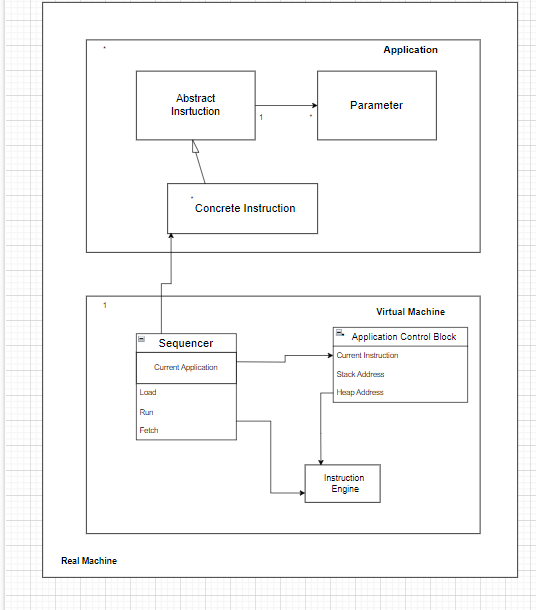
\includegraphics[scale=0.8]{images/first/virtual_machine.png}
\caption{ساختار الگوی \lr{Virtual Machine}}
\end{figure}